% ============================================================
% 讲义 — 人教版高一必修2 第8章 立体几何初步
% 编译命令：xelatex -interaction=nonstopmode 高一必修2_第8章_立体几何初步.tex
% ============================================================
\documentclass[12pt, a4paper]{ctexart}
\usepackage[margin=2.2cm]{geometry}
\usepackage{amsmath, amssymb, amsthm}
\usepackage{enumitem}
\usepackage{tcolorbox}
\usepackage{booktabs}
\usepackage{array}
\usepackage{fancyhdr}
\usepackage{xcolor}
\usepackage{tikz}
\usepackage{hyperref}
\usepackage{graphicx}
\usepackage{multirow}
\usepackage{pgfplots}
\pgfplotsset{compat=1.18}
\usetikzlibrary{3d, calc, arrows.meta, patterns}

% 颜色定义
\definecolor{mainblue}{RGB}{41, 98, 168}
\definecolor{lightblue}{RGB}{230, 240, 255}
\definecolor{tipgreen}{RGB}{34, 139, 87}
\definecolor{lightgreen}{RGB}{235, 250, 240}
\definecolor{warnred}{RGB}{200, 50, 50}
\definecolor{lightred}{RGB}{255, 240, 240}
\definecolor{examorange}{RGB}{210, 120, 20}
\definecolor{lightorange}{RGB}{255, 248, 235}
\definecolor{apppurple}{RGB}{120, 60, 170}
\definecolor{lightpurple}{RGB}{245, 238, 255}

% 页眉页脚
\pagestyle{fancy}
\fancyhf{}
\fancyhead[L]{\small\textcolor{mainblue}{\textbf{人教版高一必修2 · 第8章 立体几何初步}}}
\fancyhead[R]{\small\textcolor{mainblue}{立体几何初步讲义}}
\fancyfoot[C]{\small —\ \thepage\ —}
\renewcommand{\headrulewidth}{0.6pt}
\renewcommand{\headrule}{\hbox to\headwidth{\color{mainblue}\leaders\hrule height \headrulewidth\hfill}}
\renewcommand{\footrulewidth}{0pt}

% tcolorbox 样式
\newtcolorbox{knowledgebox}[1][]{%
  colback=lightblue, colframe=mainblue,
  fonttitle=\bfseries\large, title=#1,
  arc=3mm, boxrule=0.8pt,
  left=8pt, right=8pt, top=6pt, bottom=6pt
}

\newtcolorbox{tipbox}[1][]{%
  colback=lightgreen, colframe=tipgreen,
  fonttitle=\bfseries, title=#1,
  arc=2mm, boxrule=0.6pt,
  left=6pt, right=6pt, top=4pt, bottom=4pt
}

\newtcolorbox{warnbox}[1][]{%
  colback=lightred, colframe=warnred,
  fonttitle=\bfseries, title=#1,
  arc=2mm, boxrule=0.6pt,
  left=6pt, right=6pt, top=4pt, bottom=4pt
}

\newtcolorbox{examplebox}[1][]{%
  colback=lightorange, colframe=examorange,
  fonttitle=\bfseries, title=#1,
  arc=3mm, boxrule=0.8pt,
  left=8pt, right=8pt, top=6pt, bottom=6pt
}

\newtcolorbox{appbox}[1][]{%
  colback=lightpurple, colframe=apppurple,
  fonttitle=\bfseries, title=#1,
  arc=3mm, boxrule=0.8pt,
  left=8pt, right=8pt, top=6pt, bottom=6pt
}

\setCJKmainfont{Hiragino Sans GB}
\setCJKsansfont{Heiti SC}

\begin{document}

% ============ 标题页 ============
\begin{center}
{\Huge\bfseries\textcolor{mainblue}{第8章\quad 立体几何初步}}\\[12pt]
{\Large\textcolor{gray}{讲\quad 义}}\\[8pt]
\rule{0.6\textwidth}{1pt}\\[8pt]
{\normalsize 适用：人教版\quad 高一必修2\quad |\quad 课时：4课时}
\end{center}
\vspace{10pt}

% ============================================================
%   第一部分：知识点讲解
% ============================================================
\section*{\textcolor{mainblue}{一、知识点讲解}}

% -------------------- 8.1 空间几何体 --------------------
\subsection*{8.1\quad 空间几何体（棱柱、棱锥、棱台）}

\begin{knowledgebox}[【知识1】棱柱]
\textbf{定义：}有两个面互相平行，其余各面都是四边形，且每相邻两个四边形的公共边都互相平行，由这些面所围成的多面体叫做\textbf{棱柱}。

\medskip
\textbf{分类：}
\begin{itemize}[leftmargin=2em]
  \item 按底面边数：三棱柱、四棱柱、五棱柱……
  \item 按侧棱与底面关系：\textbf{直棱柱}（侧棱垂直于底面）、\textbf{斜棱柱}（侧棱不垂直于底面）。
\end{itemize}

\textbf{性质：}
\begin{enumerate}[leftmargin=2em]
  \item 侧棱都平行且相等；
  \item 两个底面是全等的多边形；
  \item 平行于底面的截面与底面全等。
\end{enumerate}

\textbf{体积公式：} $V = Sh$，其中 $S$ 为底面积，$h$ 为高。

\medskip
\textbf{侧面积（直棱柱）：} $S_{\text{侧}} = Ch$，其中 $C$ 为底面周长。

\medskip
\textbf{表面积：} $S_{\text{表}} = S_{\text{侧}} + 2S_{\text{底}}$。

\medskip
\textbf{特殊棱柱——长方体：}
设长、宽、高分别为 $a, b, c$，则体对角线长 $l = \sqrt{a^2 + b^2 + c^2}$。
\end{knowledgebox}

% 棱柱 tikz 图
\begin{center}
\begin{tikzpicture}[scale=1.0, line join=round, line cap=round]
  % 四棱柱
  \coordinate (A) at (0,0);
  \coordinate (B) at (2.5,0);
  \coordinate (C) at (3.2,1.2);
  \coordinate (D) at (0.7,1.2);
  \coordinate (A1) at (0.7,2.5);
  \coordinate (B1) at (3.2,2.5);
  \coordinate (C1) at (3.9,3.7);
  \coordinate (D1) at (1.4,3.7);
  \draw[thick, mainblue] (A) -- (B) -- (C) -- (D) -- cycle;
  \draw[thick, mainblue] (A1) -- (B1) -- (C1) -- (D1) -- cycle;
  \draw[thick, mainblue] (A) -- (A1);
  \draw[thick, mainblue] (B) -- (B1);
  \draw[thick, mainblue] (C) -- (C1);
  \draw[thick, dashed, mainblue] (D) -- (D1);
  \node[below left] at (A) {$A$};
  \node[below right] at (B) {$B$};
  \node[right] at (C) {$C$};
  \node[left] at (D) {$D$};
  \node[left] at (A1) {$A_1$};
  \node[right] at (B1) {$B_1$};
  \node[right] at (C1) {$C_1$};
  \node[left] at (D1) {$D_1$};
  \node[below] at (1.95,-0.3) {\small 四棱柱};
\end{tikzpicture}
\hspace{2cm}
\begin{tikzpicture}[scale=1.0, line join=round, line cap=round]
  % 三棱柱
  \coordinate (A) at (0,0);
  \coordinate (B) at (2.5,0);
  \coordinate (C) at (1.25,2.17);
  \coordinate (A1) at (1.2,1.5);
  \coordinate (B1) at (3.7,1.5);
  \coordinate (C1) at (2.45,3.67);
  \draw[thick, mainblue] (A) -- (B) -- (C) -- cycle;
  \draw[thick, mainblue] (A1) -- (B1) -- (C1) -- cycle;
  \draw[thick, mainblue] (A) -- (A1);
  \draw[thick, mainblue] (B) -- (B1);
  \draw[thick, dashed, mainblue] (C) -- (C1);
  \node[below left] at (A) {$A$};
  \node[below right] at (B) {$B$};
  \node[above] at (C) {$C$};
  \node[above left] at (A1) {$A_1$};
  \node[right] at (B1) {$B_1$};
  \node[above right] at (C1) {$C_1$};
  \node[below] at (1.85,-0.3) {\small 三棱柱};
\end{tikzpicture}
\end{center}

\begin{knowledgebox}[【知识2】棱锥]
\textbf{定义：}有一个面是多边形，其余各面是有一个公共顶点的三角形，由这些面所围成的多面体叫做\textbf{棱锥}。

\medskip
\textbf{分类：}按底面边数分为三棱锥（四面体）、四棱锥、五棱锥……

\medskip
\textbf{正棱锥：}底面是正多边形，且顶点在底面上的射影是底面中心的棱锥。

\textbf{正棱锥性质：}
\begin{enumerate}[leftmargin=2em]
  \item 各侧棱相等；
  \item 各侧面是全等的等腰三角形；
  \item 斜高（侧面三角形的高）相等。
\end{enumerate}

\textbf{体积公式：} $V = \dfrac{1}{3}Sh$，其中 $S$ 为底面积，$h$ 为高。

\medskip
\textbf{侧面积（正棱锥）：} $S_{\text{侧}} = \dfrac{1}{2}Cl$，其中 $C$ 为底面周长，$l$ 为斜高。
\end{knowledgebox}

% 棱锥 tikz 图
\begin{center}
\begin{tikzpicture}[scale=1.0, line join=round, line cap=round]
  \coordinate (A) at (0,0);
  \coordinate (B) at (3,0);
  \coordinate (C) at (3.5,1.3);
  \coordinate (D) at (0.5,1.3);
  \coordinate (S) at (1.75,3.5);
  \coordinate (O) at (1.75,0.65);
  \draw[thick, mainblue] (A) -- (B) -- (C) -- (D) -- cycle;
  \draw[thick, mainblue] (A) -- (S);
  \draw[thick, mainblue] (B) -- (S);
  \draw[thick, mainblue] (C) -- (S);
  \draw[thick, dashed, mainblue] (D) -- (S);
  \draw[dashed, tipgreen] (S) -- (O);
  \fill (O) circle (1.5pt);
  \node[below left] at (A) {$A$};
  \node[below right] at (B) {$B$};
  \node[right] at (C) {$C$};
  \node[left] at (D) {$D$};
  \node[above] at (S) {$S$};
  \node[below right, tipgreen] at (O) {$O$};
  \node[below] at (1.75,-0.3) {\small 四棱锥};
\end{tikzpicture}
\end{center}

\begin{knowledgebox}[【知识3】棱台]
\textbf{定义：}用一个平行于棱锥底面的平面去截棱锥，底面与截面之间的部分叫做\textbf{棱台}。

\medskip
\textbf{性质：}
\begin{itemize}[leftmargin=2em]
  \item 上、下底面是相似多边形；
  \item 各侧棱延长后交于一点（原棱锥顶点）。
\end{itemize}

\textbf{体积公式：}
\[
V = \frac{1}{3}h\!\left(S_1 + S_2 + \sqrt{S_1 S_2}\right)
\]
其中 $S_1, S_2$ 分别为上、下底面积，$h$ 为高。
\end{knowledgebox}

% 棱台 tikz 图
\begin{center}
\begin{tikzpicture}[scale=1.0, line join=round, line cap=round]
  \coordinate (A) at (0,0);
  \coordinate (B) at (3,0);
  \coordinate (C) at (3.5,1.3);
  \coordinate (D) at (0.5,1.3);
  \coordinate (A1) at (0.8,0.5);
  \coordinate (B1) at (2.2,0.5);
  \coordinate (C1) at (2.5,1.5);
  \coordinate (D1) at (1.1,1.5);
  \draw[thick, mainblue] (A) -- (B) -- (C) -- (D) -- cycle;
  \draw[thick, mainblue] (A1) -- (B1) -- (C1) -- (D1) -- cycle;
  \draw[thick, mainblue] (A) -- (A1);
  \draw[thick, mainblue] (B) -- (B1);
  \draw[thick, mainblue] (C) -- (C1);
  \draw[thick, dashed, mainblue] (D) -- (D1);
  \draw[thick, dashed, mainblue] (D) -- (A1);
  \node[below left] at (A) {$A$};
  \node[below right] at (B) {$B$};
  \node[right] at (C) {$C$};
  \node[left] at (D) {$D$};
  \node[above left] at (A1) {$A_1$};
  \node[above right] at (B1) {$B_1$};
  \node[above right] at (C1) {$C_1$};
  \node[above left] at (D1) {$D_1$};
  \node[below] at (1.75,-0.3) {\small 四棱台};
\end{tikzpicture}
\end{center}

\begin{warnbox}[易错提醒]
\begin{itemize}[leftmargin=2em]
  \item 棱锥的体积是同底等高棱柱体积的 $\dfrac{1}{3}$，不是 $\dfrac{1}{2}$。
  \item 棱台体积公式中有三项 $S_1 + S_2 + \sqrt{S_1 S_2}$，不能遗漏 $\sqrt{S_1 S_2}$ 项。
  \item 棱台的侧棱\textbf{不平行}，它们延长后交于一点。
\end{itemize}
\end{warnbox}

% -------------------- 8.2 三视图与直观图 --------------------
\subsection*{8.2\quad 三视图与直观图}

\begin{knowledgebox}[【知识4】三视图]
\textbf{三视图}由主视图（正视图）、俯视图、侧视图（左视图）组成。

\textbf{投影规律（长对正、高平齐、宽相等）：}
\begin{enumerate}[leftmargin=2em]
  \item 正视图与俯视图的\textbf{长}对正；
  \item 正视图与侧视图的\textbf{高}平齐；
  \item 俯视图与侧视图的\textbf{宽}相等。
\end{enumerate}
\end{knowledgebox}

\begin{center}
\begin{tikzpicture}[scale=0.9]
  \draw[thick, mainblue] (0,0) rectangle (2.5,2);
  \node[above, mainblue] at (1.25,2) {\textbf{正视图}};
  \draw[thick, tipgreen] (3.5,0) rectangle (5.5,2);
  \node[above, tipgreen] at (4.5,2) {\textbf{侧视图}};
  \draw[thick, examorange] (0,-1) rectangle (2.5,-3);
  \node[below, examorange] at (1.25,-1) {\textbf{俯视图}};
  \draw[->, dashed, gray] (2.5,1) -- (3.5,1);
  \node[above, gray] at (3,1) {\small 高平齐};
  \draw[->, dashed, gray] (1.25,0) -- (1.25,-1);
  \node[left, gray] at (1.25,-0.5) {\small 长对正};
\end{tikzpicture}
\end{center}

\begin{knowledgebox}[【知识5】斜二测画法（直观图）]
\textbf{斜二测画法规则：}
\begin{enumerate}[leftmargin=2em]
  \item 在原图形中建立直角坐标系 $xOy$；
  \item 画直观图时，$x'$ 轴与 $y'$ 轴的夹角为 $45°$（或 $135°$）；
  \item 平行于 $x$ 轴的线段长度\textbf{不变}；
  \item 平行于 $y$ 轴的线段长度变为原来的 $\dfrac{1}{2}$。
\end{enumerate}

\textbf{面积关系：} $S_{\text{直观图}} = \dfrac{\sqrt{2}}{4} \, S_{\text{原图}}$。
\end{knowledgebox}

\begin{center}
\begin{tikzpicture}[scale=1.0]
  \draw[thick, mainblue] (0,0) rectangle (2,2);
  \node[below] at (1,0) {\small 原图};
  \draw[->, thick, gray] (2.5,1) -- (3.5,1);
  \draw[thick, examorange] (4,0) -- (6,0) -- (6.7,1) -- (4.7,1) -- cycle;
  \node[below] at (5.35,0) {\small 直观图};
  \draw[->, thick] (4,-0.3) -- (6.5,-0.3) node[right] {$x'$};
  \draw[->, thick] (4,-0.3) -- (5,1.3) node[left] {$y'$};
\end{tikzpicture}
\end{center}

\begin{warnbox}[易错提醒]
\begin{itemize}[leftmargin=2em]
  \item 只有与 $y$ 轴平行方向的长度缩短为原来的一半，与 $x$ 轴平行方向的长度不变。
  \item 原图中的直角在直观图中一般不再是直角。
  \item 直观图面积与原图面积之比为 $\dfrac{\sqrt{2}}{4}$，不要记反。
\end{itemize}
\end{warnbox}

% -------------------- 8.3 空间点、线、面位置关系 --------------------
\subsection*{8.3\quad 空间点、线、面位置关系}

\begin{knowledgebox}[【知识6】平面的基本性质（公理）]
\textbf{公理1：}如果一条直线上的两个点在一个平面内，那么这条直线在此平面内。

\textbf{公理2：}过不在同一条直线上的三点，有且只有一个平面。

\textbf{公理3：}如果两个不重合的平面有一个公共点，那么它们有且只有一条过该点的公共直线。

\medskip
\textbf{推论：}
\begin{enumerate}[leftmargin=2em]
  \item 经过一条直线和直线外一点，有且只有一个平面；
  \item 经过两条相交直线，有且只有一个平面；
  \item 经过两条平行直线，有且只有一个平面。
\end{enumerate}
\end{knowledgebox}

\begin{knowledgebox}[【知识7】空间中线与线、线与面、面与面的位置关系]
\begin{center}
\renewcommand{\arraystretch}{1.3}
\begin{tabular}{|c|c|c|}
\hline
\textbf{关系} & \textbf{位置} & \textbf{说明} \\
\hline
\multirow{3}{*}{线与线} & 共面相交 & 有且只有一个公共点 \\
\cline{2-3}
 & 共面平行 & 无公共点，在同一平面内 \\
\cline{2-3}
 & 异面 & 无公共点，不在任何同一平面内 \\
\hline
\multirow{2}{*}{线与面} & 平行 & 无公共点 \\
\cline{2-3}
 & 相交 & 有且只有一个公共点 \\
\hline
\multirow{2}{*}{面与面} & 平行 & 无公共点 \\
\cline{2-3}
 & 相交 & 有一条公共直线 \\
\hline
\end{tabular}
\end{center}

\textbf{异面直线所成的角：}过空间任意一点分别作两条异面直线的平行线，这两条相交直线所成的锐角（或直角）叫做异面直线所成的角，范围为 $(0°, 90°]$。
\end{knowledgebox}

\begin{warnbox}[易错提醒]
\begin{itemize}[leftmargin=2em]
  \item "没有公共点"不一定是平行，还可能是异面！
  \item 两条直线垂直不一定相交——异面垂直也存在。
  \item 判断异面直线时，关键是说明"不能在同一平面内"。
\end{itemize}
\end{warnbox}

% -------------------- 8.4 平行关系 --------------------
\subsection*{8.4\quad 平行关系的判定与性质}

\begin{knowledgebox}[【知识8】线面平行]
\textbf{判定定理：}平面外一条直线与此平面内的一条直线平行，则该直线与此平面平行。
\[\boxed{a \not\subset \alpha,\; b \subset \alpha,\; a \parallel b \;\Longrightarrow\; a \parallel \alpha}\]

\textbf{性质定理：}一条直线与一个平面平行，则过该直线的任一平面与此平面的交线与该直线平行。
\[\boxed{a \parallel \alpha,\; a \subset \beta,\; \alpha \cap \beta = b \;\Longrightarrow\; a \parallel b}\]
\end{knowledgebox}

\begin{center}
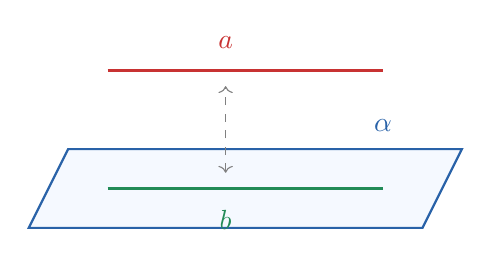
\begin{tikzpicture}[scale=1.0]
  \fill[lightblue, opacity=0.4] (-2,-0.5) -- (3,-0.5) -- (3.5,0.5) -- (-1.5,0.5) -- cycle;
  \draw[thick, mainblue] (-2,-0.5) -- (3,-0.5) -- (3.5,0.5) -- (-1.5,0.5) -- cycle;
  \node[mainblue] at (2.5,0.8) {$\alpha$};
  \draw[thick, tipgreen] (-1,0) -- (2.5,0);
  \node[tipgreen, below] at (0.5,-0.15) {$b$};
  \draw[thick, warnred] (-1,1.5) -- (2.5,1.5);
  \node[warnred, above] at (0.5,1.65) {$a$};
  \draw[<->, gray, dashed] (0.5,0.2) -- (0.5,1.3);
\end{tikzpicture}
\end{center}

\begin{knowledgebox}[【知识9】面面平行]
\textbf{判定定理：}一个平面内的两条\textbf{相交}直线与另一个平面平行，则这两个平面平行。
\[\boxed{a \subset \alpha,\; b \subset \alpha,\; a \cap b = P,\; a \parallel \beta,\; b \parallel \beta \;\Longrightarrow\; \alpha \parallel \beta}\]

\textbf{性质定理：}
\begin{enumerate}[leftmargin=2em]
  \item 两个平面平行，则其中一个平面内的直线平行于另一个平面。
  \item 两个平行平面与第三个平面相交，则两条交线平行。
\end{enumerate}
\[\boxed{\alpha \parallel \beta,\; \gamma \cap \alpha = a,\; \gamma \cap \beta = b \;\Longrightarrow\; a \parallel b}\]
\end{knowledgebox}

% -------------------- 8.5 垂直关系 --------------------
\subsection*{8.5\quad 垂直关系的判定与性质}

\begin{knowledgebox}[【知识10】线面垂直]
\textbf{定义：}如果一条直线与一个平面内的\textbf{任意}一条直线都垂直，则称该直线与该平面\textbf{垂直}。

\medskip
\textbf{判定定理：}一条直线与一个平面内的两条\textbf{相交}直线都垂直，则该直线与此平面垂直。
\[\boxed{a \subset \alpha,\; b \subset \alpha,\; a \cap b = P,\; l \perp a,\; l \perp b \;\Longrightarrow\; l \perp \alpha}\]

\textbf{性质定理：}
\begin{enumerate}[leftmargin=2em]
  \item 垂直于同一个平面的两条直线平行：$a \perp \alpha,\; b \perp \alpha \;\Longrightarrow\; a \parallel b$。
  \item 一条直线垂直于一个平面，则它垂直于平面内的\textbf{所有}直线。
\end{enumerate}
\end{knowledgebox}

\begin{center}
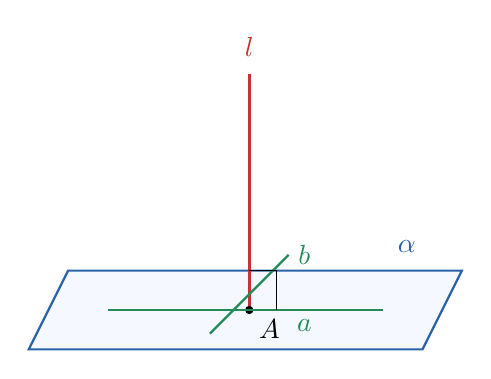
\begin{tikzpicture}[scale=1.0]
  \fill[lightblue, opacity=0.4] (-2,-0.5) -- (3,-0.5) -- (3.5,0.5) -- (-1.5,0.5) -- cycle;
  \draw[thick, mainblue] (-2,-0.5) -- (3,-0.5) -- (3.5,0.5) -- (-1.5,0.5) -- cycle;
  \node[mainblue] at (2.8,0.8) {$\alpha$};
  \draw[very thick, warnred] (0.8,0) -- (0.8,3);
  \node[warnred, above] at (0.8,3.1) {$l$};
  \fill (0.8,0) circle (1.5pt);
  \node[below right] at (0.8,0) {$A$};
  \draw[thick, tipgreen] (-1,0) -- (2.5,0);
  \draw[thick, tipgreen] (0.3,-0.3) -- (1.3,0.7);
  \node[tipgreen, below] at (1.5,0) {$a$};
  \node[tipgreen, right] at (1.3,0.7) {$b$};
  \draw (0.8,0.5) -- (1.15,0.5) -- (1.15,0);
\end{tikzpicture}
\end{center}

\begin{knowledgebox}[【知识11】面面垂直]
\textbf{定义：}两个平面相交，如果所成的二面角是直二面角（$90°$），则称这两个平面\textbf{互相垂直}。

\medskip
\textbf{判定定理：}一个平面过另一个平面的垂线，则这两个平面垂直。
\[\boxed{l \perp \alpha,\; l \subset \beta \;\Longrightarrow\; \alpha \perp \beta}\]

\textbf{性质定理：}两个平面垂直，则在一个平面内垂直于交线的直线垂直于另一个平面。
\[\boxed{\alpha \perp \beta,\; \alpha \cap \beta = m,\; a \subset \alpha,\; a \perp m \;\Longrightarrow\; a \perp \beta}\]
\end{knowledgebox}

% -------------------- 8.6 空间角 --------------------
\subsection*{8.6\quad 空间角（线面角与二面角）}

\begin{knowledgebox}[【知识12】线面角]
\textbf{定义：}平面的一条斜线与它在平面上的\textbf{射影}所成的锐角，叫做该直线与平面所成的角。

\medskip
\textbf{取值范围：}
\begin{itemize}[leftmargin=2em]
  \item 直线平行于平面或在平面内，线面角为 $0°$；
  \item 斜线与平面所成的角 $\theta \in (0°, 90°)$；
  \item 直线垂直于平面，线面角为 $90°$。
\end{itemize}
\end{knowledgebox}

\begin{center}
\begin{tikzpicture}[scale=1.0]
  \fill[lightblue, opacity=0.3] (0,0) -- (4,0) -- (4,0.5) -- (0,0.5) -- cycle;
  \draw[thick, mainblue] (0,0) -- (4,0);
  \node[mainblue, right] at (4,0) {$\alpha$};
  \draw[thick, warnred] (1.5,0) -- (3,2.5);
  \node[warnred, above right] at (3,2.5) {$l$};
  \draw[thick, tipgreen, dashed] (1.5,0) -- (3,0);
  \node[tipgreen, below] at (2.25,0) {射影};
  \draw[thick, examorange] (1.5,0) + (0.7,0) arc (0:59:0.7);
  \node[examorange, right] at (2.1,0.4) {$\theta$};
  \fill (1.5,0) circle (1.5pt);
  \node[below left] at (1.5,0) {$H$};
\end{tikzpicture}
\end{center}

\begin{knowledgebox}[【知识13】二面角]
\textbf{定义：}从一条直线出发的两个半平面所组成的图形叫做\textbf{二面角}，这条直线叫做二面角的\textbf{棱}，这两个半平面叫做二面角的\textbf{面}。

\medskip
\textbf{二面角的平面角：}以二面角的棱上任意一点为端点，在两个面内分别作垂直于棱的两条射线，这两条射线所成的角叫做二面角的\textbf{平面角}。二面角的大小等于其平面角的大小。

\medskip
\textbf{取值范围：} $[0°, 180°]$。
\end{knowledgebox}

\begin{center}
\begin{tikzpicture}[scale=1.0]
  \draw[very thick, gray] (0,0) -- (5,0);
  \node[gray, below] at (2.5,0) {\small 棱 $l$};
  \fill[lightblue, opacity=0.4] (0,0) -- (2.5,2.5) -- (5,0) -- cycle;
  \draw[thick, mainblue] (0,0) -- (2.5,2.5) -- (5,0);
  \node[mainblue] at (2.8,1.8) {$\alpha$};
  \fill[lightgreen, opacity=0.4] (0,0) -- (2.5,-1.8) -- (5,0) -- cycle;
  \draw[thick, tipgreen] (0,0) -- (2.5,-1.8) -- (5,0);
  \node[tipgreen] at (2.8,-1.2) {$\beta$};
  \draw[thick, warnred] (1,0) -- (1,1.5);
  \draw[thick, warnred] (1,0) -- (2.2,-0.7);
  \draw[thick, warnred] (1,0.75) arc (0:-35:0.75);
  \node[warnred, right] at (1.6,0.6) {$\theta$};
  \draw (1,0) -- (1.3,0) -- (1.3,0.3);
  \draw (1,0) -- (1.15,-0.24);
\end{tikzpicture}
\end{center}

\begin{tipbox}[求空间角的方法总结]
\begin{enumerate}[leftmargin=2em]
  \item \textbf{找}：在图形中找到所求的角（注意射影的确定）。
  \item \textbf{证}：证明所找的角就是所求的角。
  \item \textbf{算}：在直角三角形中用三角函数或余弦定理计算角的大小。
\end{enumerate}
关键是\textbf{找射影}和\textbf{构造直角三角形}。
\end{tipbox}

% ============================================================
%   第二部分：例题精讲
% ============================================================
\section*{\textcolor{examorange}{二、例题精讲}}

% ───── 例题 1 ─────
\begin{examplebox}[【例题1】正三棱柱的体积与表面积]
一个正三棱柱的底面边长为 $4$，侧棱长为 $6$。求该棱柱的全面积和体积。
\end{examplebox}

\textbf{解：}

底面为正三角形，边长 $a = 4$。

底面积 $S_{\text{底}} = \dfrac{\sqrt{3}}{4} a^2 = \dfrac{\sqrt{3}}{4} \times 16 = 4\sqrt{3}$。

侧面积 $S_{\text{侧}} = 3 \times 4 \times 6 = 72$。

全面积 $S_{\text{表}} = 2S_{\text{底}} + S_{\text{侧}} = 8\sqrt{3} + 72$。

体积 $V = S_{\text{底}} \cdot h = 4\sqrt{3} \times 6 = 24\sqrt{3}$。

\begin{tipbox}[方法总结]
正棱柱的全面积 $=$ 两个底面积 $+$ 侧面积。正三角形面积公式 $S = \dfrac{\sqrt{3}}{4}a^2$ 在棱柱、棱锥问题中经常使用。
\end{tipbox}

\vspace{6pt}

% ───── 例题 2 ─────
\begin{examplebox}[【例题2】正四棱锥的体积]
正四棱锥的底面边长为 $6$，侧面与底面所成二面角为 $60°$。求该棱锥的高和体积。
\end{examplebox}

\textbf{解：}

底面为正方形，边长 $a = 6$，底面积 $S = 36$。

取底面中心 $O$，底面一边的中点 $M$，则 $OM = \dfrac{a}{2} = 3$。

设棱锥顶点为 $P$，连接 $PM$（斜高），$PO$（高）。

侧面与底面所成二面角的平面角为 $\angle PMO = 60°$。

在 $\mathrm{Rt}\triangle POM$ 中：
\[
\tan 60° = \frac{PO}{OM} \implies PO = 3\tan 60° = 3\sqrt{3}
\]

体积 $V = \dfrac{1}{3}Sh = \dfrac{1}{3} \times 36 \times 3\sqrt{3} = 36\sqrt{3}$。

\begin{center}
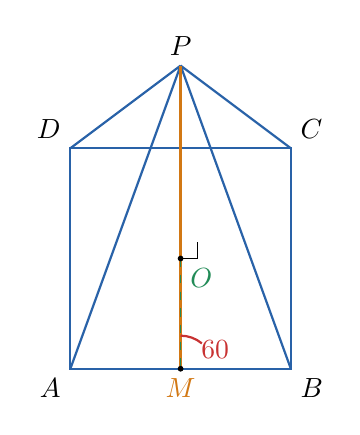
\begin{tikzpicture}[scale=0.7]
  \coordinate (A) at (0,0);
  \coordinate (B) at (4,0);
  \coordinate (C) at (4,4);
  \coordinate (D) at (0,4);
  \coordinate (O) at (2,2);
  \coordinate (P) at (2,5.5);
  \coordinate (M) at (2,0);
  \draw[thick, mainblue] (A) -- (B) -- (C) -- (D) -- cycle;
  \draw[thick, mainblue] (A) -- (P) (B) -- (P) (C) -- (P) (D) -- (P);
  \draw[dashed, tipgreen] (O) -- (P);
  \draw[thick, examorange] (M) -- (P);
  \draw[dashed, tipgreen] (O) -- (M);
  \fill (O) circle (1.5pt);
  \fill (M) circle (1.5pt);
  \node[below right, tipgreen] at (O) {$O$};
  \node[below, examorange] at (M) {$M$};
  \node[above] at (P) {$P$};
  \node[below left] at (A) {$A$};
  \node[below right] at (B) {$B$};
  \node[above right] at (C) {$C$};
  \node[above left] at (D) {$D$};
  \draw[thick, warnred] (2,0) + (0,0.6) arc (90:50:0.6);
  \node[warnred, right] at (2.2,0.35) {$60°$};
  \draw (2,2) -- (2.3,2) -- (2.3,2.3);
\end{tikzpicture}
\end{center}

\begin{tipbox}[方法总结]
正棱锥问题的关键是利用底面中心 $O$、底面边中点 $M$ 与顶点 $P$ 构成的直角三角形 $\triangle POM$。侧面与底面所成二面角的平面角就是 $\angle PMO$。
\end{tipbox}

\vspace{6pt}

% ───── 例题 3 ─────
\begin{examplebox}[【例题3】棱台的体积]
一个正四棱台的上底面边长为 $2$，下底面边长为 $4$，高为 $3$。求其体积。
\end{examplebox}

\textbf{解：}

上底面积 $S_1 = 2^2 = 4$，下底面积 $S_2 = 4^2 = 16$。

$\sqrt{S_1 S_2} = \sqrt{4 \times 16} = 8$。

\begin{align*}
V &= \frac{1}{3}h\!\left(S_1 + S_2 + \sqrt{S_1 S_2}\right) \\
  &= \frac{1}{3} \times 3 \times (4 + 16 + 8) \\
  &= 28
\end{align*}

\begin{tipbox}[方法总结]
棱台体积公式可以理解为"上底面积 $+$ 下底面积 $+$ 几何平均值"之和乘以 $\dfrac{h}{3}$。切记不要遗漏 $\sqrt{S_1 S_2}$ 项。
\end{tipbox}

\vspace{6pt}

% ───── 例题 4 ─────
\begin{examplebox}[【例题4】线面平行的证明]
在三棱锥 $P$--$ABC$ 中，$D$、$E$ 分别是 $AB$、$AC$ 的中点。求证：$DE \parallel$ 平面 $PBC$。

\begin{center}
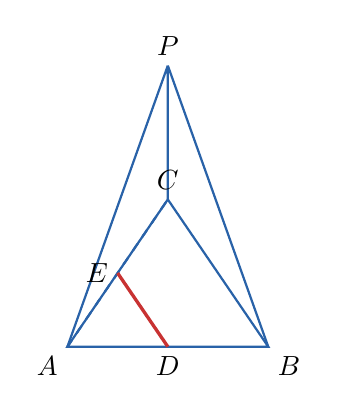
\begin{tikzpicture}[scale=0.85]
  \coordinate (A) at (0,0);
  \coordinate (B) at (3,0);
  \coordinate (C) at (1.5,2.2);
  \coordinate (P) at (1.5,4.2);
  \coordinate (D) at (1.5,0);
  \coordinate (E) at (0.75,1.1);
  \draw[thick, mainblue] (A) -- (B) -- (C) -- cycle;
  \draw[thick, mainblue] (A) -- (P) (B) -- (P) (C) -- (P);
  \draw[thick, dashed, mainblue] (A) -- (C);
  \draw[thick, warnred, very thick] (D) -- (E);
  \node[below left] at (A) {$A$};
  \node[below right] at (B) {$B$};
  \node[above] at (C) {$C$};
  \node[above] at (P) {$P$};
  \node[below] at (D) {$D$};
  \node[left] at (E) {$E$};
\end{tikzpicture}
\end{center}
\end{examplebox}

\textbf{证明：}

$\because$ $D$、$E$ 分别是 $AB$、$AC$ 的中点，

$\therefore$ 在 $\triangle ABC$ 中，$DE \parallel BC$，$DE = \dfrac{1}{2}BC$（三角形中位线定理）。

$\because$ $DE \not\subset$ 平面 $PBC$，$BC \subset$ 平面 $PBC$，

$\therefore$ 由线面平行判定定理，$DE \parallel$ 平面 $PBC$。 \qed

\begin{tipbox}[方法总结]
证明线面平行的常用方法：
\begin{enumerate}[leftmargin=2em]
  \item 在目标平面内找一条与已知直线平行的直线（利用中位线、平行四边形对边平行等）；
  \item 利用面面平行的性质。
\end{enumerate}
\end{tipbox}

\vspace{6pt}

% ───── 例题 5 ─────
\begin{examplebox}[【例题5】线面垂直的证明]
在四面体 $P$--$ABC$ 中，$PA \perp$ 平面 $ABC$，$AB \perp BC$。求证：$BC \perp$ 平面 $PAB$。

\begin{center}
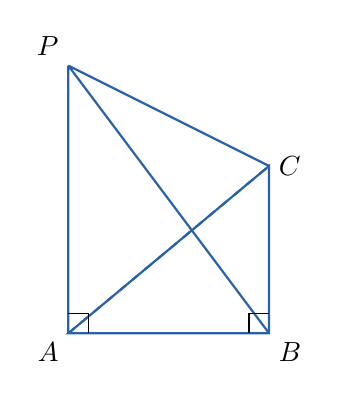
\begin{tikzpicture}[scale=0.85]
  \coordinate (A) at (0,0);
  \coordinate (B) at (3,0);
  \coordinate (C) at (3,2.5);
  \coordinate (P) at (0,4);
  \draw[thick, mainblue] (A) -- (B) -- (C) -- cycle;
  \draw[thick, mainblue] (A) -- (P) (B) -- (P) (C) -- (P);
  \draw[thick, dashed, mainblue] (A) -- (C);
  \draw (2.7,0) -- (2.7,0.3) -- (3,0.3);
  \draw (0.3,0) -- (0.3,0.3) -- (0,0.3);
  \node[below left] at (A) {$A$};
  \node[below right] at (B) {$B$};
  \node[right] at (C) {$C$};
  \node[above left] at (P) {$P$};
\end{tikzpicture}
\end{center}
\end{examplebox}

\textbf{证明：}

$\because$ $PA \perp$ 平面 $ABC$，$BC \subset$ 平面 $ABC$，

$\therefore$ $PA \perp BC$（线面垂直的性质）。

又 $\because$ $AB \perp BC$（已知），

$PA \cap AB = A$，$PA \subset$ 平面 $PAB$，$AB \subset$ 平面 $PAB$，

$\therefore$ 由线面垂直判定定理，$BC \perp$ 平面 $PAB$。 \qed

\vspace{6pt}

% ───── 例题 6 ─────
\begin{examplebox}[【例题6】面面垂直的证明]
在四棱锥 $P$--$ABCD$ 中，底面 $ABCD$ 是正方形，$PA \perp$ 底面 $ABCD$。求证：平面 $PBD \perp$ 平面 $PAC$。
\end{examplebox}

\textbf{证明：}

设正方形对角线 $AC$ 与 $BD$ 交于点 $O$。

$\because$ $ABCD$ 为正方形，$\therefore$ $AC \perp BD$。

$\because$ $PA \perp$ 底面 $ABCD$，$BD \subset$ 底面 $ABCD$，

$\therefore$ $PA \perp BD$。

$\because$ $AC \perp BD$，$PA \perp BD$，$AC \cap PA = A$，

$AC \subset$ 平面 $PAC$，$PA \subset$ 平面 $PAC$，

$\therefore$ $BD \perp$ 平面 $PAC$。

$\because$ $BD \subset$ 平面 $PBD$，

$\therefore$ 平面 $PBD \perp$ 平面 $PAC$（面面垂直判定定理）。 \qed

\begin{tipbox}[方法总结]
面面垂直的证明思路：
\begin{enumerate}[leftmargin=2em]
  \item 在一个平面内找一条直线垂直于另一个平面（先证线面垂直）；
  \item 利用面面垂直判定定理得出结论。
\end{enumerate}
\end{tipbox}

\vspace{6pt}

% ───── 例题 7 ─────
\begin{examplebox}[【例题7】线面角的计算]
在正方体 $ABCD$--$A_1B_1C_1D_1$ 中，棱长为 $a$。求 $A_1C$ 与底面 $ABCD$ 所成的角。
\end{examplebox}

\textbf{解：}

连接 $AC$，则 $AC$ 是 $A_1C$ 在底面 $ABCD$ 上的射影（因为 $A_1A \perp$ 底面）。

$\angle A_1CA$ 即为 $A_1C$ 与底面所成的角。

在正方体中：
\begin{itemize}[leftmargin=2em]
  \item $A_1A = a$（高），
  \item $AC = \sqrt{2}\,a$（底面正方形对角线）。
\end{itemize}

在 $\mathrm{Rt}\triangle A_1AC$ 中：
\[
\tan \angle A_1CA = \frac{A_1A}{AC} = \frac{a}{\sqrt{2}\,a} = \frac{1}{\sqrt{2}} = \frac{\sqrt{2}}{2}
\]

$\therefore$ $\angle A_1CA = \arctan \dfrac{\sqrt{2}}{2}$。

\begin{center}
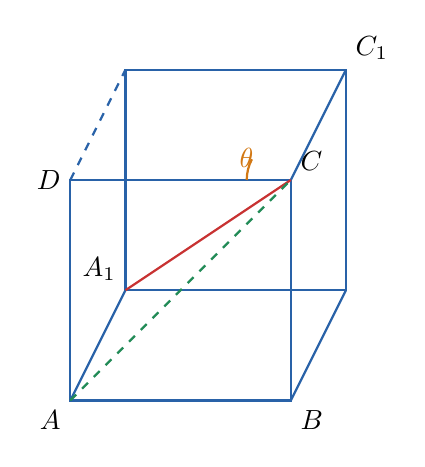
\begin{tikzpicture}[scale=0.7]
  \coordinate (A) at (0,0);
  \coordinate (B) at (4,0);
  \coordinate (C) at (4,4);
  \coordinate (D) at (0,4);
  \coordinate (A1) at (1,2);
  \coordinate (B1) at (5,2);
  \coordinate (C1) at (5,6);
  \coordinate (D1) at (1,6);
  \draw[thick, mainblue] (A) -- (B) -- (C) -- (D) -- cycle;
  \draw[thick, mainblue] (A1) -- (B1) -- (C1) -- (D1) -- cycle;
  \draw[thick, mainblue] (A) -- (A1) (B) -- (B1) (C) -- (C1);
  \draw[thick, dashed, mainblue] (D) -- (D1);
  \draw[thick, warnred] (A1) -- (C);
  \draw[thick, tipgreen, dashed] (A) -- (C);
  \draw[thick, examorange] (4,4) + (-0.8,0) arc (180:152:0.8);
  \node[examorange, left] at (3.5,4.4) {$\theta$};
  \node[below left] at (A) {$A$};
  \node[below right] at (B) {$B$};
  \node[above right] at (C) {$C$};
  \node[left] at (D) {$D$};
  \node[above left] at (A1) {$A_1$};
  \node[above right] at (C1) {$C_1$};
\end{tikzpicture}
\end{center}

\begin{tipbox}[方法总结]
求线面角的步骤：
\begin{enumerate}[leftmargin=2em]
  \item 找到斜线在平面上的射影（过斜线上一点作平面的垂线，垂足与斜足连线即为射影）；
  \item 斜线与射影所成的锐角即为线面角；
  \item 在含线面角的直角三角形中计算。
\end{enumerate}
\end{tipbox}

\vspace{6pt}

% ───── 例题 8 ─────
\begin{examplebox}[【例题8】二面角的计算]
在正方体 $ABCD$--$A_1B_1C_1D_1$ 中，棱长为 $1$。求二面角 $A$--$BD_1$--$A_1$ 的余弦值。
\end{examplebox}

\textbf{解：}

以 $D$ 为原点，$\vec{DA}$、$\vec{DC}$、$\vec{DD_1}$ 分别为 $x$、$y$、$z$ 轴建立空间直角坐标系。

$D(0,0,0)$，$A(1,0,0)$，$B(1,1,0)$，$A_1(1,0,1)$，$D_1(0,0,1)$。

棱 $BD_1$：$\vec{BD_1} = (-1,-1,1)$。

\textbf{求平面 $ABD_1$ 的法向量：}

$\vec{BA} = (0,-1,0)$，$\vec{BD_1} = (-1,-1,1)$。

$\vec{n_1} = \vec{BA} \times \vec{BD_1} = \begin{vmatrix} \vec{i} & \vec{j} & \vec{k} \\ 0 & -1 & 0 \\ -1 & -1 & 1 \end{vmatrix} = (-1, 0, -1)$

取 $\vec{n_1} = (1, 0, 1)$。

\textbf{求平面 $A_1BD_1$ 的法向量：}

$\vec{BA_1} = (0,-1,1)$，$\vec{BD_1} = (-1,-1,1)$。

$\vec{n_2} = \vec{BA_1} \times \vec{BD_1} = \begin{vmatrix} \vec{i} & \vec{j} & \vec{k} \\ 0 & -1 & 1 \\ -1 & -1 & 1 \end{vmatrix} = (0, -1, -1)$

取 $\vec{n_2} = (0, 1, 1)$。

\textbf{求二面角：}

$\cos \theta = \dfrac{|\vec{n_1} \cdot \vec{n_2}|}{|\vec{n_1}||\vec{n_2}|} = \dfrac{|0 + 0 + 1|}{\sqrt{2} \cdot \sqrt{2}} = \dfrac{1}{2}$

$\therefore$ 二面角 $A$--$BD_1$--$A_1 = 60°$。

\begin{tipbox}[方法总结]
用向量法求二面角：分别求两个半平面的法向量 $\vec{n_1}$、$\vec{n_2}$，则二面角 $\theta$ 满足
$\cos\theta = \dfrac{|\vec{n_1} \cdot \vec{n_2}|}{|\vec{n_1}||\vec{n_2}|}$。
注意取绝对值后对应的是锐角或直角的二面角；若需判断钝角，需结合几何图形分析法向量的方向。
\end{tipbox}

\vspace{6pt}

% ───── 例题 9 ─────
\begin{examplebox}[【例题9】综合题：棱锥中的垂直与体积]
在三棱锥 $P$--$ABC$ 中，$PA \perp$ 平面 $ABC$，$\angle BCA = 90°$，$BC = CA = 2$，$PA = 2$。

(1) 求证：$BC \perp$ 平面 $PAC$；

(2) 求三棱锥 $P$--$ABC$ 的体积。

\begin{center}
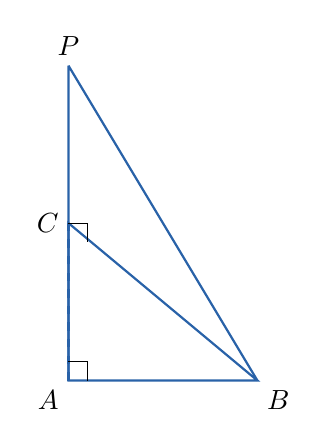
\begin{tikzpicture}[scale=0.8]
  \coordinate (A) at (0,0);
  \coordinate (B) at (3,0);
  \coordinate (C) at (0,2.5);
  \coordinate (P) at (0,5);
  \draw[thick, mainblue] (A) -- (B) -- (C) -- cycle;
  \draw[thick, mainblue] (A) -- (P) (B) -- (P) (C) -- (P);
  \draw[thick, dashed, mainblue] (A) -- (C);
  \draw (0.3,0) -- (0.3,0.3) -- (0,0.3);
  \draw (0.3,2.2) -- (0.3,2.5) -- (0,2.5);
  \node[below left] at (A) {$A$};
  \node[below right] at (B) {$B$};
  \node[left] at (C) {$C$};
  \node[above] at (P) {$P$};
\end{tikzpicture}
\end{center}
\end{examplebox}

\textbf{解：}

\textbf{(1) 证明：}

$\because$ $PA \perp$ 平面 $ABC$，$BC \subset$ 平面 $ABC$，

$\therefore$ $PA \perp BC$。

$\because$ $\angle BCA = 90°$，$\therefore$ $BC \perp AC$。

$PA \cap AC = A$，$PA \subset$ 平面 $PAC$，$AC \subset$ 平面 $PAC$，

$\therefore$ $BC \perp$ 平面 $PAC$。 \qed

\textbf{(2) 求体积：}

$\triangle ABC$ 为等腰直角三角形，$\angle BCA = 90°$，$BC = CA = 2$。

$S_{\triangle ABC} = \dfrac{1}{2} \times 2 \times 2 = 2$。

$V = \dfrac{1}{3} S_{\triangle ABC} \cdot PA = \dfrac{1}{3} \times 2 \times 2 = \dfrac{4}{3}$。

\vspace{6pt}

% ───── 例题 10 ─────
\begin{examplebox}[【例题10】正四棱锥中求线面角]
正四棱锥 $S$--$ABCD$ 的底面边长为 $4$，高 $SO = 3$。求侧棱 $SA$ 与底面 $ABCD$ 所成的角。
\end{examplebox}

\textbf{解：}

$O$ 为底面正方形 $ABCD$ 的中心。

$SA$ 在底面上的射影为 $OA$。

$\angle SAO$ 即为 $SA$ 与底面所成的角。

$OA = \dfrac{1}{2}AC = \dfrac{1}{2} \times 4\sqrt{2} = 2\sqrt{2}$。

在 $\mathrm{Rt}\triangle SAO$ 中：
\[
\tan \angle SAO = \frac{SO}{OA} = \frac{3}{2\sqrt{2}} = \frac{3\sqrt{2}}{4}
\]

$\therefore$ $\angle SAO = \arctan \dfrac{3\sqrt{2}}{4}$。

% ============================================================
%   第三部分：应用题
% ============================================================
\section*{\textcolor{apppurple}{三、应用题}}

\begin{appbox}[【应用1】金字塔形建筑]
一座金字塔形建筑的底面是边长为 $20$ 米的正方形，侧面与底面所成的二面角为 $60°$。求这座建筑的高度和四面斜墙的总面积。
\end{appbox}

\textbf{解：}

底面正方形中心到边中点的距离 $OM = 10$ 米。

设金字塔高为 $h$，侧面与底面所成二面角的平面角为 $\angle SMO = 60°$。

$\tan 60° = \dfrac{h}{10}$，$\therefore$ $h = 10\sqrt{3} \approx 17.3$ 米。

斜高 $l = SM = \dfrac{OM}{\cos 60°} = \dfrac{10}{0.5} = 20$ 米。

每个侧面面积 $= \dfrac{1}{2} \times 20 \times 20 = 200$ 平方米。

四面斜墙总面积 $= 4 \times 200 = 800$ 平方米。

\vspace{6pt}

\begin{appbox}[【应用2】棱台形蓄水池]
一个棱台形蓄水池的上底面为边长 $6$ 米的正方形，下底面为边长 $4$ 米的正方形，深 $3$ 米。求该蓄水池的容积。若每立方米水重 $1$ 吨，水池最多能装多少吨水？
\end{appbox}

\textbf{解：}

上底面积 $S_1 = 6^2 = 36$，下底面积 $S_2 = 4^2 = 16$。

$\sqrt{S_1 S_2} = \sqrt{36 \times 16} = 24$。

\begin{align*}
V &= \frac{1}{3}h\!\left(S_1 + S_2 + \sqrt{S_1 S_2}\right) \\
  &= \frac{1}{3} \times 3 \times (36 + 16 + 24) \\
  &= 76 \text{（立方米）}
\end{align*}

最多能装 $76$ 吨水。

\vspace{6pt}

\begin{appbox}[【应用3】三视图还原与体积]
某几何体的三视图如下：正视图为矩形（宽 $4$，高 $3$），侧视图为矩形（宽 $3$，高 $3$），俯视图为三角形（底 $4$，高 $3$）。判断该几何体的形状并求其体积。
\end{appbox}

\textbf{解：}

由俯视图为三角形知底面为三角形，由正视图和侧视图为矩形知该几何体为\textbf{直三棱柱}。

底面为直角三角形，两直角边分别为 $3$ 和 $4$（由俯视图确定），棱柱高为 $3$（由正视图高确定）。

底面积 $S = \dfrac{1}{2} \times 3 \times 4 = 6$。

体积 $V = Sh = 6 \times 3 = 18$。

\begin{center}
\begin{tikzpicture}[scale=0.8]
  \draw[thick, mainblue] (0,0) rectangle (2,1.5);
  \node[below] at (1,-0.1) {\small 正视图};
  \draw[thick, tipgreen] (3,0) -- (4.5,0) -- (4.5,1.5) -- (3,1.5) -- cycle;
  \node[below] at (3.75,-0.1) {\small 侧视图};
  \draw[thick, examorange] (5.5,0) -- (7.5,0) -- (5.5,1.5) -- cycle;
  \node[below] at (6.17,-0.1) {\small 俯视图};
\end{tikzpicture}
\end{center}

% ============================================================
%   第四部分：课堂练习
% ============================================================
\section*{\textcolor{tipgreen}{四、课堂练习}}

\begin{enumerate}[leftmargin=2em, label=\textbf{\arabic*.}]
  \item 一个正六棱柱的底面边长为 $2$，高为 $3$，求其体积和侧面积。

  \item 一个正三棱锥的底面边长为 $6$，侧面与底面所成二面角为 $60°$，求该棱锥的高和体积。

  \item 在长方体 $ABCD$--$A_1B_1C_1D_1$ 中，$AB = 3$，$BC = 4$，$AA_1 = 5$。求 $AC_1$ 的长。

  \item 在正方体 $ABCD$--$A_1B_1C_1D_1$ 中，$M$、$N$ 分别为 $BB_1$、$DD_1$ 的中点。求证：$MN \parallel$ 平面 $ABCD$。

  \item 在四棱锥 $P$--$ABCD$ 中，底面 $ABCD$ 为正方形，$PA \perp$ 底面，$PA = AB = 2$。$M$ 为 $PB$ 的中点。求证：$AM \perp PC$。

  \item 在正方体 $ABCD$--$A_1B_1C_1D_1$ 中，棱长为 $1$。求 $BD_1$ 与底面 $ABCD$ 所成角的正切值。
\end{enumerate}

\vspace{10pt}
\begin{knowledgebox}[参考答案]

\textbf{1.} 正六边形面积 $S = 6 \times \dfrac{\sqrt{3}}{4} \times 2^2 = 6\sqrt{3}$。

体积 $V = Sh = 6\sqrt{3} \times 3 = 18\sqrt{3}$。

底面周长 $C = 6 \times 2 = 12$，侧面积 $S_{\text{侧}} = 12 \times 3 = 36$。

\medskip

\textbf{2.} 底面中心到边中点距离：正三角形中心（重心）到边的距离 $= \dfrac{1}{3}$ 中线长 $= \dfrac{1}{3} \times \dfrac{\sqrt{3}}{2} \times 6 = \sqrt{3}$。

$\tan 60° = \dfrac{h}{\sqrt{3}}$，$h = \sqrt{3} \times \sqrt{3} = 3$。

底面积 $= \dfrac{\sqrt{3}}{4} \times 36 = 9\sqrt{3}$。

$V = \dfrac{1}{3} \times 9\sqrt{3} \times 3 = 9\sqrt{3}$。

\medskip

\textbf{3.} $AC_1 = \sqrt{AB^2 + BC^2 + AA_1^2} = \sqrt{9 + 16 + 25} = \sqrt{50} = 5\sqrt{2}$。

\medskip

\textbf{4.} 设正方体棱长为 $1$，以 $D$ 为原点建系：$D(0,0,0)$，$B(1,1,0)$，$B_1(1,1,1)$，$D_1(0,0,1)$。

$M$ 为 $BB_1$ 中点：$M(1,1,\frac{1}{2})$。$N$ 为 $DD_1$ 中点：$N(0,0,\frac{1}{2})$。

$\vec{MN} = (-1,-1,0)$。又 $\vec{DB} = (1,1,0)$，故 $\vec{MN} = -\vec{DB}$，即 $MN \parallel DB$。

$\because$ $MN \not\subset$ 平面 $ABCD$，$DB \subset$ 平面 $ABCD$，

$\therefore$ $MN \parallel$ 平面 $ABCD$。

\medskip

\textbf{5.} 建立坐标系：$A(0,0,0)$，$B(2,0,0)$，$C(2,2,0)$，$D(0,2,0)$，$P(0,0,2)$。

$M$ 为 $PB$ 中点，$M = (1,0,1)$。

$\vec{AM} = (1,0,1)$，$\vec{PC} = (2,2,-2)$。

$\vec{AM} \cdot \vec{PC} = 2 + 0 - 2 = 0$。

$\therefore$ $AM \perp PC$。

\medskip

\textbf{6.} $BD_1$ 在底面上的射影为 $BD$。在 $\mathrm{Rt}\triangle D_1DB$ 中（$D_1D \perp$ 底面），$D_1D = 1$，$DB = \sqrt{2}$。

$\tan \theta = \dfrac{D_1D}{DB} = \dfrac{1}{\sqrt{2}} = \dfrac{\sqrt{2}}{2}$。

\end{knowledgebox}

\vfill
\begin{center}
\small\textcolor{gray}{本讲义仅供教学参考，例题可根据学生水平调整难度。}
\end{center}

\end{document}
